% LICENSE: see LICENCE
\RequirePackage[l2tabu, orthodox]{nag}
\nonstopmode
\documentclass[a4paper,oneside,10pt]{article}

%include version control info
\input{vc.tex}

%\usepackage[bindingoffset=1.5cm,centering,includeheadfoot,margin=3cm]{geometry}

\usepackage[T1]{fontenc}
\usepackage[utf8]{inputenc}
\usepackage[pdftex]{graphicx}
%\usepackage{subfig}

\usepackage[protrusion=true,expansion=true]{microtype}

\usepackage{wrapfig}
\usepackage{fancybox}
\usepackage{shadow}
\usepackage{xspace}
\usepackage{acronym}

%\usepackage{lmodern} % new latin extended computer modern font}, use with T1
%\usepackage{pxfonts} % has replaced palatino
\usepackage{cmbright}

\usepackage{listings}

\usepackage[allowlitunits]{siunitx}
% Try $20\micro\seconds$

%\addtolength{\oddsidemargin}{-1cm}
%\addtolength{\evensidemargin}{-1cm}
%\addtolength{\textwidth}{+2cm}
%\usepackage{showframe}
%\usepackage{lastpage}
% for \pageref{LastPage}

% fancy header
\usepackage{fancyhdr}
\pagestyle{fancy}
\fancyhf{} % clear default header and footer
\fancyhead[R]{\textit{\nouppercase{\leftmark}}}
\fancyhead[C]{}
\fancyfoot[R]{\thepage}
\fancyfoot[L]{\tiny{rev~\GITAbrHash, \GITAuthorDate, \GITAuthorName.}}

\setlength{\headheight}{14pt}

\newcommand\Hrule{\noindent\rule{\linewidth}{1.5pt}}
\newcommand{\sidenote}[1]{\marginpar{\scriptsize{\textsf{#1}}}} % Bram's sidenote for comments

%\usepackage{titlesec}

\newcommand{\footnoteurl}[1]{\footnote{\url{#1}}}
\newcommand{\us}{\,\si{\micro\second}\xspace}
\newcommand{\km}{\,\si{\kilo\meter}\xspace}
\newcommand{\ms}{\,ms}
\newcommand{\dabplus}{DAB$^\mathrm{+}$\xspace}
\newcommand{\captionwidth}{0.9\textwidth}
\newcommand{\mmbtools}{\mbox{ODR-mmbTools}\xspace}

\newcommand{\filename}[1]{\texttt{#1}}

% index stuff
\usepackage{tocbibind} % Index in TOC
%\usepackage{makeidx}
%\usepackage{showidx} % show index entries in margin
%\makeindex

%\newcommand{\bib}[4]{\item{\textsc{#1}, \emph{#2}, #3\\\hspace{2em}#4}}

% ---------------------------------------------------------

\newcommand{\titleinfo}{ODR-mmbTools \\
Open-Source Software-Defined \dabplus Tools}
\author{Matthias P. Brändli}
\title{\titleinfo}


% Margins for handwritten notes
%\addtolength{\oddsidemargin}{-2cm}
%\addtolength{\evensidemargin}{-2cm}
%\addtolength{\textwidth}{-2cm}

\usepackage{xcolor}
\definecolor{Brown}{cmyk}{0,0.81,1,0.60}
\definecolor{OliveGreen}{cmyk}{0.64,0,0.95,0.40}
\definecolor{CadetBlue}{cmyk}{0.62,0.57,0.23,0}
\definecolor{lightlightgray}{cmyk}{0,0,0,0.02}
\definecolor{gray}{cmyk}{0,0,0,0.8}

\usepackage{smartdiagram}

\usepackage[pdftex,
 pdfauthor={Matthias P. Braendli},
 pdftitle={ODR-mmbTools Documentation},
 pdfsubject={},
 pdfkeywords={Digital Audio Broadcasting,DAB,single-frequency network,SFN,mmbTools,ODR-mmbTools,open-source,software-defined radio},
 pdfcreator=pdflatex]{hyperref}
\hypersetup{colorlinks, citecolor=black, filecolor=black, linkcolor=black, urlcolor=black}

% LaTeX magic: make sections have a cleardoublepage
% Useful for twoside only
%\let\stdsection\section
%\renewcommand*\section{\cleardoublepage\stdsection}

\begin{document}
\lstset{
language=C,                             % Code langugage
basicstyle=\ttfamily,                   % Code font, Examples: \footnotesize, \ttfamily
keywordstyle=\color{OliveGreen},        % Keywords font ('*' = uppercase)
commentstyle=\color{gray},              % Comments font
numbers=left,                           % Line nums position
numberstyle=\tiny,                      % Line-numbers fonts
stepnumber=1,                           % Step between two line-numbers
numbersep=5pt,                          % How far are line-numbers from code
backgroundcolor=\color{lightlightgray}, % Choose background color
frame=none,                             % A frame around the code
tabsize=2,                              % Default tab size
captionpos=b,                           % Caption-position = bottom
breaklines=true,                        % Automatic line breaking?
breakatwhitespace=false,                % Automatic breaks only at whitespace?
showspaces=false,                       % Dont make spaces visible
showtabs=false,                         % Dont make tabls visible
morekeywords={uint32_t,uint8_t,uint16_t,time_spec_t,size_t,
clock_config_t},
}
\pagestyle{empty}
\pagenumbering{roman}
 \begin{titlepage}
    \null\vfil
    \begin{flushleft}
      \huge \textbf{\titleinfo}
    \end{flushleft}
    \par
    \hrule height 4pt
    \par
    \begin{flushright}
      \large
      \textsl{Project Documentation} \par
    \end{flushright}
    \vspace{\fill}
    \vspace*{\stretch{1}}

    \begin{center}
        \Large
        Opendigitalradio\\\href{http://opendigitalradio.org}{http://opendigitalradio.org}\\2014--2017
    \end{center}
    \vspace{\fill}
    \vspace*{\stretch{2}}

    \begin{figure}[!h]
        \centering
        \parbox{2.2in}{\includegraphics[width=16em]{figures/dabtux.pdf}}
    \end{figure}

    \vspace*{1cm}
    \begin{center}
    This work is licensed under a \\
    Creative Commons Attribution-ShareAlike 4.0 International License.\\
    See \url{http://creativecommons.org/licenses/by-sa/4.0/} or LICENCE.txt
    \end{center}
 \end{titlepage}

\pagestyle{fancy}
\tableofcontents

\section*{Acronyms}
\markboth{Acronyms}{}
\addcontentsline{toc}{section}{Acronyms}
\begin{acronym}[mmbTools]
    \acro{1PPS}{One pulse per second}
    \acro{CFR}{Crest Factor Reduction}
    \acro{CIF}{Common Interleaved Frame}
    \acro{CRC}{Communications Research Centre Canada}
    \acro{DAB}{Digital Audio Broadcasting}
    \acro{DMB}{Digital Multimedia Broadcasting}
    \acro{ETI}{Ensemble Transport Interface}
    \acro{ETSI}{European Telecommunications Standards Institute}
    \acro{FIC}{Fast Information Channel}
    \acro{HE-AAC}{High Efficiency Advanced Audio Codec}
    \acro{mmbTools}{Mobile Multimedia Broadcasting Tools}
    \acro{MER}{Modulation Error Rate}
    \acro{MNSC}{Multiplex Network Signalling Channel}
    \acro{NTP}{Network Time Protocol}
    \acro{OCXO}{Oven-Controlled Crystal Oscillator}
    \acro{OFDM}{Orthogonal Frequency-Division Multiplexing}
    \acro{PAPR}{Peak-to-Average Power Ratio}
    \acro{PRBS}{Pseudo-Random Bit Sequence}
    \acro{SFN}{Single-Frequency Network}
    \acro{TCXO}{Temperature-Compensated Crystal Oscillator}
    \acro{TIST}{Timestamp field in the ETI frame}
    \acro{TM}{Transmission Mode}
    \acro{UHD}{USRP Hardware Driver}
    \acro{USRP}{Universal Software-Radio Peripheral}
\end{acronym}

\pagenumbering{arabic}
% LICENSE: see LICENCE
\section{Introductions}
This is the official documentation for the \mmbtools. These tools can be used to
experiment with digital audio broadcasting (DAB) modulation, to learn the
techniques behind it, and to set up a DAB or \dabplus transmitter.

This documentation assumes that you are already familiar with the basic concepts
of the DAB system. Understanding how the DAB transmission chain is structured is
a prerequisite for getting started with the \mmbtools. The ``DAB Bible'' by Hoeg
and Lauterbach~\cite{hoeg}, and the ``Guide to DAB standards'' from the
ETSI~\cite{etsidabguide} can be used as a starting point.

In this document, the terms ``DAB'' and ``\dabplus'' are used somewhat
interchangeably, since many parts of the transmission chain are identical
between the two variants. In most cases, ``DAB'' will be used, and ``\dabplus''
when talking about specific details about the newer version of the standard.


\section{Purpose}
The individual programs that make up the \mmbtools each have their own
documentation for command-line options and configuration settings, and the
opendigitalradio.org wiki\footnoteurl{http://opendigitalradio.org} contains many
explanations and pointers, but there is no single source of documentation
available for the whole toolset.

This document aims to fill this gap, by first outlining general concepts, then
presenting different usage scenarios, and finally, detailing a complete
transmission setup.
With this document in hand, you should be able to understand all of the elements
which go into the \mmbtools transmission chain, and how to set one up.

Please refer to the bibliography for references on any individual topic that may need
clarification, to the README files in the repositories of the tools that are
going to be presented in this guide, and if you have further questions, get in
touch with us through the mailing-list mentioned on our website.

\section{Presentation of the Tools}
\subsection{Origins}
Before we begin with technical details, first a word about the history of
the mmbTools.
In 2002, Communications Research Centre Canada\footnoteurl{http://crc.ca}
started developing a DAB multiplexer. This effort evolved through the years, and
was published in September 2009 as \mbox{CRC-DabMux} under the GPL
open-source licence.

CRC also developed a DAB modulator, called \mbox{CRC-DABMOD}, which was able to create
baseband complex quadrature (I/Q) samples from files or
streams in the ETI format. This I/Q data could then be sent to a hardware device
(for broadcast or laboratory RF measurements) using another tool. For driving
the universal software-defined radio peripherals (USRP) made by the company
Ettus Research, a ``wave player'' script was necessary to interface with GNURadio.
Only DAB Transmission Mode 2 was supported. \mbox{CRC-DABMOD} was also released
under the GPL in early 2010.

As encoders, toolame could be used for DAB, and CRC developed a closed-source
\mbox{CRC-DABPLUS} \dabplus encoder.

These three CRC-tools, and some additional services available on the now
unreachable website\footnote{There are some snapshots of the website available
    on \url{http://archive.org}.}
\url{http://mmbtools.crc.ca} were part of the \mbox{CRC-mmbTools}. These tools
made it possible to set up the first DAB transmission experiments.

In 2012, these tools received experimental support for single-frequency
networks, a functionality that has been developed by Matthias P. Brändli during
his Master's thesis\footnote{The corresponding report is available at
    \url{http://mpb.li/report.pdf}}.
Because SFNs are mainly used in TM 1, CRC subsequently released a patch to
\mbox{CRC-DABMOD} that enabled all four transmission modes.

At that point, involvement from CRC started to decline. The SFN patch was
ultimately never included in the \mbox{CRC-mmbTools}, and as time passed, the
de-facto fork on \url{http://mpb.li} was receiving more and more features.
Having two different programs with the same name made things complicated, and
so, with the approval of CRC, the tools were officially forked in February 2014,
and given the new name \mbox{ODR-mmbTools}. They are now developed by the
Opendigitalradio association.

In April 2014, the official \mbox{CRC-mmbTools} website went offline, and it has
become very difficult, if not impossible, to acquire licences for the
\mbox{CRC-DABPLUS} encoder. Luckily there is an open-source replacement
available, which was part of Google's Android source. This encoder has been
extended with the necessary \dabplus{}-specific requirements (960-transform,
error correction, framing, etc.), and now exists under the name
\mbox{fdk-aac}. The encoder \mbox{ODR-AudioEnc} can use this library to encode for
\dabplus{}.

\subsection{Included Tools}
The \mmbtools are composed of several software projects:
\mbox{ODR-DabMux}, \mbox{ODR-DabMod},
\mbox{ODR-AudioEnc}, \mbox{ODR-PadEnc}, and other scripts, bits and pieces
that are useful when setting up a transmission chain.

\begin{figure}[H]
    \centering
    \smartdiagram[bubble diagram]{
        ODR-\\ mmbTools,
        ODR-DabMux,
        ODR-DabMod,
        ODR-PadEnc,
        etisnoop,
        ODR-\\ AudioEnc,
        ODR-\\ SourceCompanion,
        ODR-\\ EncoderManager
    }
    \caption{The family of ODR-mmbTools}
    \label{fig:family_mmbTools}
\end{figure}

\subsubsection{ODR-DabMux}
ODR-DabMux implements a DAB multiplexer that combines all audio and data inputs
and outputs them in the form of a file in ETI format. This can be used offline
(i.e.~not in real time) to generate ETI data for processing later, or for use in
a real-time streaming scenario (e.g.~in a transmitter).

ODR-DabMux can read input audio or data from files (``.mp2'' for DAB, ``.dabp'' for
\dabplus), FIFOs (also called ``named pipes''), or from a network connection. This
network connection can use UDP (STI-D) or EDI.

The configuration of the multiplexer is given in a configuration file, whose
format is defined in the example files in the \verb+doc/+ folder inside the
ODR-DabMux repository.


\subsubsection{ODR-DabMod}
ODR-DabMod is a software-defined DAB modulator that receives or reads ETI data
in streams or from files, and generates modulated I/Q data which can be used for
transmission.

This I/Q data which is encoded as complex floats (32bits per complex sample) can
be written to a file or pipe, sent to a USRP device using the integrated
output for the open-source USRP Hardware Driver (UHD) or to other
software-defined radio (SDR) devices using the
SoapySDR\footnoteurl{https://github.com/pothosware/SoapySDR/wiki} library.

The output of the modulator can also be sent to a GNURadio flow-graph for
further processing, conversion or analysis using a ZeroMQ network connection.

\subsubsection{ODR-AudioEnc}
The ODR-AudioEnc encoder can be used to encode for DAB and \dabplus. It includes
a TooLAME-based MPEG encoder, and uses the \mbox{fdk-aac} library as an external
dependency to encode \dabplus{}.

The integrated TooLAME library is an MPEG-1 Layer II audio encoder that is used
to encode audio for the DAB standard.
Another encoder called twolame is not compatible with DAB even though it is more
recent than TooLAME, and cannot be used for our application.

The framing and error correction which are needed for \dabplus{}, as well as the
programme-associated data (PAD) insertion, the output EDI protocol,
and the input from Advanced Linux Sound Architecture (ALSA) were then added by
different parties.

\subsubsection{ODR-PadEnc}
This encoder is able to generate programme-associated data (PAD) that can be
injected into ODR-AudioEnc. It supports reading and encoding Dynamic Label
Segment (DLS) from a text file, and reads images from a folder for MOT Slideshow.

\subsubsection{ODR-EncoderManager}
The ODR-EncoderManager presents a web-based interface that allows the user to
create, manage and run audio and PAD encoders, and presents a HTTP API to update
Dynamic Label Segment and Slides. One instance can handle several audio encoders
simultaneously, and offers a simpler way to manage the audio encoding part of
the \dabplus transmission chain.

\subsubsection{ODR-SourceCompanion}
This tool allows using third party audio encoders with the ODR-mmbTools.

\subsubsection{etisnoop}
Etisnoop is not used in the broadcasting chain directly, but is an analysis tool
for ETI, described in the ETSI standard~\cite{etsidabeti}. ODR-DabMux can write
an ETI file that can be analysed with etisnoop. The tool can be used to verify
the multiplex signalling, the presence of data in the subchannels, and it can
decode audio into files.

Additionally, it can output statistics in YAML format, which is useful in
combination with an RTLSDR receiver and the \verb+dab2eti+ tool to monitor
transmissions.

\section{Installation of the Tools}
There are 3 ways to install the tools.

\subsection{Debian Binary Packages}
If your host is running a debian-Bullseye-based operating system and its
architecture is one of amd64, arm64 or arm/v7, then you can easily install
ODR-AudioEnc, ODR-PadEnc, ODR-DabMux and ODR-DabMod
from the ODR package repository by applying the following steps:

\begin{lstlisting}
    curl -fsSL http://debian.opendigitalradio.org/odr.asc | sudo tee /etc/apt/trusted.gpg.d/odr.asc 1>/dev/null
    curl -fsSL http://debian.opendigitalradio.org/odr.list | sudo tee /etc/apt/sources.list.d/odr.list 1>/dev/null
    apt update
    sudo apt install --yes odr-audioenc odr-padenc odr-dabmux odr-dabmod
\end{lstlisting}

\paragraph{Remarks}
The \texttt{odr-dabmux} and \texttt{odr-dabmod} packages do not include the web-based GUI Mux Manager
and the GUI and Digital Predistortion Computation engine. If you need those, then you
should look at the other 2 installation options below.

\subsection{Opendigitalradio-provided Installation Script}
This option allows you to compile and install:
\begin{itemize}
    \item the above 4 main components of the tools

    \item the web-based ODR-EncoderManager, GUI Mux Manager and GUI and Digital
        Predistortion Computation engine
    \item sample configuration files for a live broadcast
\end{itemize}

Apply the following steps:
\begin{lstlisting}
    sudo apt update && sudo apt upgrade --yes
    sudo timedatectl set-timezone your_timezone
    cd ${HOME}
    git clone https://github.com/opendigitalradio/dab-scripts.git
    bash ${HOME}/dab-scripts/install/mmbtools-get install
\end{lstlisting}

\paragraph{Remarks}
The installation script will compile the tools with all the possible features
in order to give you the greatest configuration flexibility. It will also
install and configure the \texttt{supervisord} package with the sample configuration files.

\subsection{Manual Compilation}
If you wish to compile and install some tools only and reduce disk usage by
selecting the needed features, then you should follow the instructions given
with each tool:

\begin{itemize}
    \item \texttt{odr-audioenc} https://github.com/opendigitalradio/odr-audioenc
    \item \texttt{odr-padenc} https://github.com/opendigitalradio/odr-padenc
    \item \texttt{odr-dabmux} https://github.com/opendigitalradio/odr-dabmux
    \item \texttt{odr-dabmod} https://github.com/opendigitalradio/odr-dabmod
\end{itemize}

% vim: spl=en spell tw=80 et

\section{Interfacing the Tools}
\subsection{Files and Pipes}
The first versions of these tools used files and pipes to exchange data. For
offline generation of a multiplex or a modulated I/Q, it is possible to
generate all files separately, one after the other.

Here is an example to generate a two-minute ETI file for a multiplex containing two programmes:
\begin{itemize}
    \item one DAB programme at 128kbps, encoded with toolame-dab
    \item one \dabplus{} programme at 88kbps, encoded with fdk-aac-dabplus
\end{itemize}

We assume that the audio data for the two programmes is located in uncompressed
48kHz WAV in the files \filename{prog1.wav} and \filename{prog2.wav}. The first step
is to encode the audio. The DAB programme is encoded to \filename{prog1.mp2} using:
\begin{lstlisting}
toolame -b 128 prog1.wav prog1.mp2
\end{lstlisting}

The DAB+ programme is encoded to \filename{prog2.dabp}. The extension
\filename{.dabp} is arbitrary, but since the framing is not the same as for
other AAC encoded audio, it makes sense to use a special extension. The command
is:
\begin{lstlisting}
dabplus-enc -i prog2.wav -b 88 -a o prog2.dabp
\end{lstlisting}

These resulting files can then be used with ODR-DabMux to create an ETI file.
ODR-DabMux supports many options, which makes it much more practical to set
the configuration using a file than using very long command lines. Here is a short
file that can be used for the example, which will be saved as \filename{2programmes.mux}:
\begin{lstlisting}
general {
    dabmode 1
    nbframes 5000
}
remotecontrol { telnetport 0 }
ensemble {
    id 0x4fff
    ecc 0xec ; Extended Country Code

    local-time-offset auto
    international-table 1
    label "mmbtools"
    shortlabel "mmbtools"
}
services {
    srv-p1 { label "Prog1" }
    srv-p2 { label "Prog2" }
}
subchannels {
    sub-p1 {
        type audio ; MPEG
        inputfile "prog1.mp2"
        bitrate 128
        id 10
        protection 5
    }
    sub-p2 {
        type dabplus
        inputfile "prog2.dabp"
        bitrate 88
        id 1
        protection 1
    }
}
components {
    comp-p1 {
        label Prog1
        service srv-p1
        subchannel sub-p1
    }
    comp-p2 {
        label Prog2
        service srv-p2
        subchannel sub-p2
    }
}
outputs { output1 "file://myfirst.eti?type=raw" }
\end{lstlisting}

This file defines two components, that each link one service and one
subchannel. The IDs and different protection settings are also defined.

The bitrates defined in the subchannels must correspond to the bitrate set at the encoder.

The duration of the ETI file is limited by the \lstinline{nbframes 5000} setting. Each frame
corresponds to $24$\ms, and therefore $120 / 0.024 = 5000$ frames are needed
for $120$ seconds.

The output is written to the file \filename{myfirst.eti} in the ETI(NI) format. Please
see Appendix~\ref{etiformat} for more options.

To run the multiplexer, run:
\begin{lstlisting}
odr-dabmux -e 2programmes.mux
\end{lstlisting}

This will generate the file \filename{myfirst.eti}, which will be $5000 * 6144
\approx 30$\si{MB} in size.

Congratulations! You have just created your first DAB multiplex! With the configuration file,
adding more programmes is easy. More information is available in the \filename{doc/example.mux}

\subsection{Over the Network}
\subsubsection{Authentication Support}

\section{Usage Scenarios}
\subsection{Experimentation}
\subsubsection{Creation of Non-Realtime Multiplex}
The creation of a ETI file containing two programmes, one DAB and one
\dabplus{} is covered in section \ref{sec-files}.

\subsubsection{Modulation of ETI for Offline Processing}
The ETI file generated before can then be used with ODR-DabMod to generate a
file containing I/Q samples. Here, we must chose between using the command line
or the configuration file. For a very simple example, using the command line
makes sense, but for more advanced features it is preferable to use a
configuration file. For illustration, we will present both.

To modulate the file \texttt{myfirst.eti} into \texttt{myfirst.iq}, with the
default options, the command is simply

\begin{lstlisting}
odr-dabmod myfirst.eti -f myfirst.iq
\end{lstlisting}

This will create a file containing 16-bit interleaved I/Q at $2048000$ samples
per second. The transmission mode is defined by the ETI file.

The equivalent configuration file would be
\begin{lstlisting}
[input]
transport=file
source=myfirst.eti

[output]
output=file

[fileoutput]
filename=myfirst.iq
\end{lstlisting}

This is a very minimal file that defines only the necessary settings equivalent
to the above command line options. The configuration file however supports more
options that the command line, and becomes easier to manager once the set
becomes more complex. It is best to use the example configuration availble in
the \texttt{doc/} folder.

\subsection{Interfacing Hardware Devices}
\subsubsection{Ettus USRP}
ODR-DabMod integrates support for the UHD library that can interface with all
USRP devices from Ettus. The following configuration file illustrates how to
send the \texttt{myfirst.eti} over a USRP B200 on channel 13C:

\begin{lstlisting}
[remotecontrol]
telnet=1
telnetport=2121

[input]
transport=file
source=myfirst.eti
loop=1

[modulator]
gainmode=2
digital_gain=0.8

[firfilter]
enabled=1
filtertapsfile=simple_taps.txt

[output]
output=uhd

[uhdoutput]
master_clock_rate=32768000
type=b200
txgain=40
channel=13C
\end{lstlisting}

This example also shows more options that the example for the file output:

\begin{itemize}
    \item \texttt{remotecontrol telnet=1} enables the Telnet server that can be
        used to set parameters while the modulator is running.
    \item \texttt{loop=1} rewinds the input file when the end is reached. The
        same ETI file will be transmitted over and over.
    \item \texttt{gainmode=2} sets the GainMode to VAR, which reduces
        overshoots in the output.
    \item \texttt{digital\_gain=0.8} reduces the output sample deviation, to
        reduce compression in the USRP.
    \item \texttt{firfilter enabled=1} enables an additional FIR filter to
        improve the spectrum mask.
    \item \texttt{master\_clock\_rate=32768000} sets the USRP internal clock to
        a multiple of $2048000$, which is required if we want to use the native
        DAB sample rate.
    \item \texttt{txgain=40} Sets the analog transmit gain of the USRP to 40dB,
        which is specific to the B200.
\end{itemize}

Some of these options are not necessary for the system to work, but they
improve the performance.

\subsubsection{Other Hardware}

\subsection{Audio sources}
\subsubsection{Using Existing Web-Streams}
\subsubsection{Encoders at Programme Originator Studios}

\subsection{Single-Frequency Networks}

% LICENSE: see LICENCE
\section{Data Features}
\subsection{Programme-Associated Data}
It is possible to encode Dynamic Label Segment and Slideshow using ODR-PadEnc,
and to inject the PAD data into the audio encoder.

ODR-AudioEnc and ODR-PadEnc need to be launched with the same PAD socket
identifier, and they will be able to communicate. The PAD length specifies the
amount of data that is taken away from audio and used for PAD. Valid values are
6, and the range 8 to 196. When not transmitting slides, small PAD lengths
are perfectly suitable. When using slides, it is better to use values around 30.
Higher lengths will of course accelerate the transmission of the slide at the
expense of reduced audio quality during the transmission time.

ODR-PadEnc will itself only take DLS and slides from files on the
system it runs on.
If your playout system is able to push updates using FTP, you will need to
configure and FTP server to present the right folder.

A more modern approach is offered by ODR-EncoderManager, which will not only
configure and run your encoders, but also present you an HTTP API to update DLS
and upload slides. More information is available in its README.

\subsection{FIG 1 Labels and FIG 2 Extended Labels}
The specification offers two ways to carry ensemble, service and component
labels: through FIG 1 and through FIG 2, specified in clauses 5.2.2.2 and 5.2.2.3
of ETSI EN 300 401~\cite{etsidab}.

Most receivers are only able to show FIG 1 Labels encoded in the Complete EBU
Latin character set (defined in ETSI TS 101 756 clause
5.2~\cite{etsidabtables}). Some are able to display Unicode FIG 1 Labels,
encoded either in UTF-8 or UCS-2, and, as of early 2019, receiver support for
FIG 2 Extended Labels is practically absent.

The main downside of carrying Unicode FIG 1 Labels is the length limitation: 16
bytes will only encode eight characters in alphabets that require two bytes per
character. FIG 2 supports up to 32 bytes labels to alleviate this.

The intention is that new ensembles in countries requiring labels in non-latin
alphabets transmit only FIG 2 Extended Labels, whereas currently operating
ensembles keep transmitting FIG 1 Labels. This entices receiver manufacturers to
support FIG 2 without impacting functionality of receivers currently in use.
Transmitting both FIG 1 and FIG 2 is discouraged by the specification.

The way FIG 2 is encoded has been redefined, which is why ODR-DabMux supports
two variants: FIG 2 with character flag being the old variant, and FIG 2 with
text control that will become the default variant.

\subsection{Announcements}
The ODR-DabMux multiplexer supports the insertion of FIG 0/18 and FIG 0/19 that
are used to define and trigger announcements according to ETSI TR 101 496-2
Clause 3.6.8~\cite{etsitr1014962}.
An example configuration is available in the ODR-DabMux repository, in
\texttt{doc/advanced.mux}.

The best known application for announcements is traffic information, but other
kinds of announcements can also be signalled. ODR-DabMux allows triggering the
announcements through the telnet and ZMQ remote control interfaces.

\subsection{Service Linking}
ODR-DabMux also supports the ability to inform receivers about other ways to
receive a given service, through the FIGs 0/6, 0/21 and 0/24. FIG 0/6
communicates the identifiers of services linked together, 0/21 informs the
receiver about other frequencies, and 0/24 includes information about other DAB
ensembles carrying the linked service.
Their interaction is outlined in ETSI TS 103 176~\cite{etsits103176}.

You will find an example configuration in the ODR-DabMux repository, in
\texttt{doc/servicelinking.mux}.

% vim: spl=en spell tw=80 et

% LICENSE: see LICENCE
\section{System Environment}

In this section, we describe the system configuration requirements for the
continuous operation of the tools. The production environment differs in some
respects to those used for experimentation and in laboratory testing. Monitoring,
automatic recovery (in case of errors) and resilience are crucial in 24/7
operations. The term \emph{production environment} will be used here to refer to
such use.

\subsection{Launching the tools}

Services running in a production environment are usually administered remotely,
and must be able to run without user intervention, or connection. Traditionally,
such services are implemented (in UNIX terminology) as `daemons'. These are
started and stopped using the init system contained within the distribution.
The ODR-mmbTools cannot daemonise themselves, so this requires another approach:

\paragraph{Screen multiplexer}
A simple approach is to use a screen multiplexer such as \emph{GNU Screen} or
\emph{tmux} - either of these can be used to launch a session from which the
user can detach, and later re-attach at will - leaving the tools running within
it. Please see the relevant manpages for more information.

Although a screen multiplexer alone permits the tools to run without a user
being connected, it alone cannot automatically restart failed processes, and it
is unable to provide warnings in the case of a problem.

The dab-scripts, already mentioned in \ref{usingexistingwebstreams}, can be
employed to monitor the processes and (if necessary) restart them, and send an
alert via email.

\paragraph{supervisord}
As an alternative to using the scripts, the execution of the tools can also be
carried out by a dedicated tool. \texttt{supervisor}\footnote{\url{http://supervisord.org}}
is (as the name implies) such a tool.

Once installed, supervisor reads its configuration file in \texttt{/etc/supervisor.conf}
and launches the processes that are to be monitored. Each process is described
by a file. The following example assumes the tools are run as user \texttt{odr},
and that the multiplex configuration is in \texttt{/home/odr/config.mux}, and
that ODR-DabMux is to be launched.The logs of ODR-DabMux is written to the
specified log files.

\begin{lstlisting}
[program:ODR-DabMux]
command=odr-dabmux config.mux
directory=/home/odr
user=odr
autostart=true
autorestart=true
stdout_logfile=/home/odr/logs/mux.out.log
stderr_logfile=/home/odr/logs/mux.err.log
\end{lstlisting}

Once this configuration has been added to the supervisor configuration, the
settings have to be re-read using:
\begin{lstlisting}
supervisorctl reread
\end{lstlisting}

In order for supervisor to start managing and running this process, it needs to
be added:

\begin{lstlisting}
supervisorctl add ODR-DabMux
\end{lstlisting}

Setting up more processes (such as any of the other tools) can be easily
achieved by customising the configuration template above. Examples are provided
in the \texttt{mmbtools-aux} repository, under the \texttt{supervisor} folder -
these need to be changed to reflect the paths that are in use on your system.

supervisor also includes a small web-server that can display the state of the
managed processes. It is enabled with the \verb+[inet_http_server]+ setting in
the configuration file.

\subsection{Logging}
Collecting information about events is essential within a production environment.
This information is essential forensic analysis, and tracing sources of trouble.
This is achieved through the logging of important messages that can be sent by
the tools.

ODR-DabMux and ODR-DabMod both support logging to standard error, to a file and
to the system logger \texttt{syslog}. Logging to syslog is the most flexible
approach; log information can be forwarded over the network to a
centralised logging server - where logs can then be filtered according to the
priority of each message. Both tools log to the LOCAL0 facility which in turn
can be redirected into an ODR-mmbtools specific log file.

\sidenote{Describe rsyslog configuration}

In order to avoid the log files from becomming undesirably large, \texttt{logrotate}
should be set to rotate the files automatically.

\sidenote{Describe logrotate configuration}


\subsection{Timing}
The ODR-mmbTools require the system time to be accurate in order for them to
function correctly - this is especially important when running a SFN, but is
also important for standalone transmitters when in a production environment. It
is also important to remember that most receivers have a clock that is
synchronised to the clock time which is being transmitted by the multiplex to
which it has been tuned.

The system needs to run a NTP client that synchronises the system time over the
network. Correct synchronisation can be checked using the \texttt{lpeers}
command of the \texttt{ntpq} tool. The magnitude of the offset should be below
$10$\ms.

The performance of the NTP synchronisation should also be monitored permanently
during operation.


\subsection{Monitoring using munin}

The Munin\footnote{\url{http://munin-monitoring.org/}} monitoring tool can
create graphs for essential system health parameters. It can also send emails
if values transgress the defined bounds - this assists the operator in the
assessment of system status, as well as the health of the services.

In addition to basic system measurements like CPU, RAM and disk usage, NTP
synchronisation, disk and network performance (and much more besides), there
are also custom data sources for ODR-DabMux;

These data sources include ZMQ input buffer monitoring (buffer level, underruns
and overruns) and the peak audio input levels (mono, or stereo). It
can be installed by copying \verb+doc/stats_dabmux_multi.py+ to
\texttt{/etc/munin/plugins.d}. They require that the ODR-DabMux management
server is enabled in the configuration, and will automatically generate the
graphs for the subchannels used in the configuration.


\subsection{Real-time Scheduling}

As a general principle, it is prudent not to run tools (that do not need superuser
privileges) as the \texttt{root} user. The same principle also applies to the
ODR-mmbTools, but care has to be taken that the tools can still request real-time
scheduling when it is needed.

This is achieved by adding the following to \texttt{/etc/security/limits.conf},
assuming the tools are run under the user \texttt{odr}.

\begin{lstlisting}
odr          -       rtprio          65
odr          -       nice           -10
\end{lstlisting}

If you have installed JACK with real-time privileges, you may find this has
already been configured for the `audio' group, written as \texttt{@audio}, which
should suffice providing your desired user is a member of the `audio' group.

\subsection{Accessing the USRP as Non-root}

Superuser privileges are not required to access USB-connected USRP devices, but
sometimes the system lacks the configuration to enable normal users to
communicate with the device.
In that case, it is necessary to add a rule file for \texttt{udev}. This file is
included in the UHD sources, but might not have been automatically installed.
The file is called \texttt{10-uhd-usrp.rules}, should be placed into
\texttt{/etc/udev/rules.d/} and should contain

{ \footnotesize
\begin{verbatim}
#USRP1
SUBSYSTEMS=="usb", ATTRS{idVendor}=="fffe", ATTRS{idProduct}=="0002", MODE:="0666"
#B100
SUBSYSTEMS=="usb", ATTRS{idVendor}=="2500", ATTRS{idProduct}=="0002", MODE:="0666"
#B200
SUBSYSTEMS=="usb", ATTRS{idVendor}=="2500", ATTRS{idProduct}=="0020", MODE:="0666"
\end{verbatim}
}

% vim: spl=en spell tw=80 et

% LICENSE: see LICENCE
\section{Single-Frequency Networks}
\subsection{Requirements}
The DAB standard has been designed to enable the creation of transmission
networks where several transmitters share the same frequency, and send the same
signal synchronously. Such networks are called ``Single-Frequency Networks''.
Each transmitter needs to be fed the same multiplex stream, which must include
timing information required for synchronisation. This timing information implies
that a time reference must be installed at each transmitter.

The requirements for a SFN can therefore be summarised in three points:
\begin{itemize}
    \item The signal must be \emph{identical} for each transmitter. This
        requires a common multiplexers, and a distribution network that carries
        the ETI to all modulators.
    \item All transmitters must transmit on the \emph{same frequency}. The modulators
        require a frequency reference.
    \item The signal must be transmitted at the \emph{same time}, which requires
        a time reference at each site. It also implies that the ETI stream must
        contain timestamps.
\end{itemize}


The figure~\ref{fig:txchain-sfn} shows a SFN setup with two transmitters.

\begin{figure}[h]
    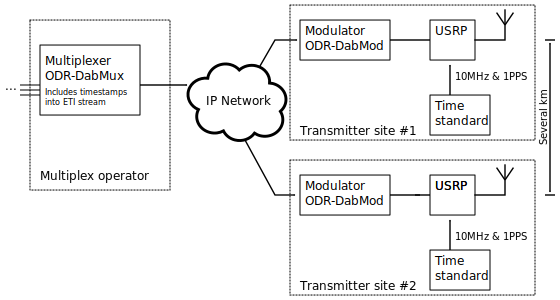
\includegraphics[width=\textwidth]{figures/txchain-sfn.pdf}
    \caption{This outline for a SFN shows two transmission sites.}
    \label{fig:txchain-sfn}
\end{figure}

\sidenote{Explain requirements on system time, NTP}

\subsection{Multiplexer Configuration}
On the ODR-DabMux configuration, there are not many options that are specific to
an SFN setup.
Most importantly, the timestamp feature must be enabled using the ``tist'' option in
the ``general'' section.

Furthermore, it is recommended to use the ZeroMQ transport between the
multiplexer and the modulators, which can be enabled in the ``outputs'' section.
Care has to be taken to have an output that slows ODR-DabMux down to nominal
rate. The ZeroMQ output alone does not enforce this. The following listing shows
the relevant options we just covered.

\begin{lstlisting}
general {
    tist true
    ...
}

...

outputs {
    ; Accept connections on all interfaces, on port 9100
    zmq  "zmq+tcp://*:9100"
    ; This throttles muxing down to nominal rate
    throttle "simul://"
}
\end{lstlisting}

\subsection{Modulator Configuration}
Since the modulator has to ensure that the three SFN requirements are satisfied,
its configuration is more complex.

We will assume, in this explanation, that one of the following USRP devices is
used: USRP2, USRP B100, USRP B200. Other devices also support the necessary time
and frequency synchronisation, but they have not been well tested. These USRP
devices can accept different sources for the reference clock:
\begin{itemize}
    \item The default ``internal'' source uses the non-disciplined
        clock generator inside the USRP. It is not suitable for SFN.
    \item The ``external'' source corresponds to the SMA connector on
        the USRP. A 10MHz signal from an external source must be connected to
        it.
    \item The optional GPSDO that can be mounted inside the USRP, and is
        selected as source with the ``gpsdo'' setting.
\end{itemize}

For the time reference, the ``pps\_source'' option is used. Possible values are
``none'', ``external'' and ``gpsdo'', with analogous meaning as for the
reference clock.

In case the USRP is connected to external references, the relevant configuration
would be as follows:

\begin{lstlisting}
[uhdoutput]
refclk_source=external
pps_source=external
\end{lstlisting}

These settings alone do not tell the modulator to enable synchronisation of the
transmission, they only select how the USRP is configured. To enable timestamp
decoding and the frame synchronisation logic in ODR-DabMod, the following
settings must also be set:

\begin{lstlisting}
[delaymanagement]
synchronous=1

; The constant offset to be added to the TIST, in seconds
offset=2.0
\end{lstlisting}

The ``offset'' setting deserves some further explanations. The ETI data stream
contains TIST information, from which a time-stamp for each ETI frame can be
derived. Each ETI frame ($24$\ms interval) is therefore associated with a
precise point in time that defines the time of transmission of the corresponding
transmission frame.\footnote{It is slightly more complex, because one
    transmission frame is composed of several ETI frames in some
    transmission modes, but the principle stays the same. It suffices for this
    explanation that we can derive the transmission time from the TIST
information.} The TIST information is set to current time at ETI frame
generation, and does not take in account the propagation delay across the
distribution network. Therefore, we need to add an offset, called $\delta$, to
the TIST to define transmission time.

\[
t_{transmission} = t_{TIST} + \delta
\]

If this offset is set to a higher value, there will be a bigger delay (measured
in absolute time) between the point in time a frame is multiplexed and the point
in time the frame is transmitted. More frames therefore will be buffered in
the ODR-DabMod input, increasing robustness against network latency
fluctuations.

The offset already has two functions: it compensates for network delay and
allows a trade-off between delay and robustness. But it also serves a third
purpose: When doing coverage planning for an SFN, it is necessary to be able to
control the relative delay between transmitters in the order of milliseconds.
This tuning of relative delay is included in the ``offset'' setting. We can
therefore rewrite the above equation as:

\[
    t_{transmission} = t_{TIST} + \delta_{network} + \delta_{planning}
\]
\[
    \delta_{offset} = \delta_{network} + \delta_{planning}
\]

When using the ZeroMQ input, the \verb+max_frames_queued+ setting must be
large enough to contain enough ETI frames to accommodate the offset.

\subsection{Using ODR LEA-M8F GPSDO board}

The ODR GPSDO board integrating a u-blox LEA-M8F module can be used as time and
frequency reference for the USRP B200. \sidenote{TODO: Add Picture}
The board design is available on the Opendigitalradio website, with
a bill of materials describing how to source the components. The PCB itself can
be manufactured in any PCB fab.

The module includes the correct pin header so that it can be mounted directly
onto the USRP B200, but also includes footprints for SMA connectors for other
usages. Communication between the PC and the GPS is possible through USB or over
UART through the B200.

The u-blox LEA-M8F module is a GPS disciplined TCXO module, with a one-pulse per
second and a reference clock output at a frequency of $30.72$ MHz. This is
different than what the normal USRP firmware expects.

Because the UART communication protocol and the reference clock frequency are
different than for the GPSDO units Ettus supports, a modified version of UHD is
necessary. This version includes new UHD sensors, used by ODR-DabMod to verify
that the GPSDO is locked properly, and different configuration settings for the
clock management PLL inside the USRP, making the USRP compatible to the
$30.72$MHz reference clock frequency.

The modified UHD version is available on the ODR GitHub\footnote{
    \url{http://www.github.com/Opendigitalradio/uhd.git}} and is used in place
of Ettus' UHD.

ODR-DabMod can be configured as follows:
\begin{lstlisting}
[uhdoutput]
refclk_source=gpsdo
pps_source=gpsdo
behaviour_refclk_lock_lost=crash
max_gps_holdover_time=600
\end{lstlisting}


\subsection{Using Ettus GPSDO}
When using the GPSDO from Ettus, which is a Jackson Labs Firefly module, no
special UHD version needs to be installed.

The configuration is:
\begin{lstlisting}
[uhdoutput]
refclk_source=gpsdo-ettus
pps_source=gpsdo
behaviour_refclk_lock_lost=crash
max_gps_holdover_time=600
\end{lstlisting}

% vim: spl=en spell tw=80 et

\appendix

\section{CRC-DABMUX ETI file formats}
\label{etiformat}
CRC-DABMUX supports three output formats for the ETI stream, that have been described on the mmbTools forum
website.\footnote{\url{http://mmbtools.crc.ca/component/option,com\_fireboard/Itemid,55/func,view/id,4/catid,13/\#28}}

The three formats are called \emph{framed}, \emph{streamed} and \emph{raw}.

The \emph{framed} format is used for saving a finite ETI stream into a file. Each frame does not contain any padding, and the
format can be described as follows:
\begin{lstlisting} 
uint32_t nbFrames
// for each frame
  uint16_t frameSize
  uint8_t data[frameSize]
\end{lstlisting}

When streaming data, in which case the number of frames is not known in advance, the \emph{streamed} format can be used.
This format is identical to the first one except for the missing \texttt{nbFrames}.
\begin{lstlisting} 
// for each frame
  uint16_t frameSize
  uint8_t data[frameSize]
\end{lstlisting}

The \emph{raw} format corresponds to ETI(NI), where each frame has a constant size of 6144 Bytes. The padding in this
case is necessary.
\begin{lstlisting} 
// for each frame
  uint8_t data[6144]
\end{lstlisting}

In order to select the format, the following syntax for the \texttt{-O} option is used:
\texttt{-O file://filename?type=format}, where \texttt{format} is one of \verb+framed+, \verb+streamed+ or
\verb+raw+.




\end{document}

% vim: spl=en spell tw=80 et
